%!TEX root = /Users/andy/Documents/Academics/Dissertation/thesis.tex

\chapter{Bending waves during \textit{Caenorhabditis elegans} locomotion are driven and organized by proprioceptive coupling }


\section{Introduction}
\lettrine{H}{ow neural circuits give rise to coordinated rhythmic behaviors} such as locomotion remains a fundamental question in systems neuroscience 
\citep{delcomyn_neural_1980}. Classic studies sought the neuromuscular 
basis of locomotion in aquatic swimmers such as lamprey and leech \citep{marder_principles_1996,kristan_rhythmic_1976,cohen_neuronal_1980,friesen_neuronal_1978,ermentrout_frequency_1984}. In these systems, the concept of a Central Pattern Generator (CPG) is commonly evoked to explain rhythmic behavior \citep{delcomyn_neural_1980,marder_principles_1996}. The CPG hypothesis is supported by observations that motor neurons in each body segment continue to exhibit rhythmic activity even after pruning all inputs \citep{kristan_rhythmic_1976,cohen_neuronal_1980,pearce_intersegmental_1984}.




Whereas a CPG could produce rhythmic behavior, motor circuits still need to respond to sensory 
inputs to deliver precise and flexible control of body movement \citep{delcomyn_neural_1980}. In leech, muscle activity can be coordinated among segments by sensory feedback even after cutting neuronal couplings between segments \citep{yu_sensory_1999}. In \textit{Drosophila larva}, specific classes of mechanosensory neurons that tile the whole body contribute to organizing peristaltic waves during locomotion \citep{hughes_sensory_2007,song_peripheral_2007,cheng_role_2010}. In \textit{C. 
elegans}, the shape and speed of bending waves adapt to the mechanical load imposed by the 
environment \citep{fang-yen_biomechanical_2010,berri_forward_2009}, and mutations in a mechanosensitive channel (TRP-4) acting in the DVA 
interneuron perturb the amplitude and frequency of body undulation \citep{li_c._2006}.


Here, we sought a biophysical characterization of the role of proprioceptive feedback in the \textit{C. elegans} locomotory circuit by combining microfluidics and optical neurophysiology \citep{liewald_optogenetic_2008,chronis_microfluidics_2007,zhang_multimodal_2007,clark_temporal_2007,lockery_artificial_2008}. We discovered that stretch-sensitive coupling between adjacent body regions represents the key mechanism for driving bending waves along the worm body during forward locomotion.





\section{Results}
\subsection{The bending of one body region requires the bending of its anterior neighbor}

\textit{C. elegans} moves forward by propagating dorsal-ventral body bending waves from head to tail. 
The detailed kinematics of bending waves can be quantified using the time-varying curvature 
measured at each point along the body centerline over time (Fig.~\ref{fig:proc1}a). To compare data from different worms, we normalized distance along the centerline by measuring fractional distance 
from head to tail (head $=0$; tail $=1$). Each body region alternates between positive (red) and 
negative (blue) curvature and bands of curvature propagate from head to tail as shown in a 
kymograph (Fig.~\ref{fig:proc1}b). 




\begin{FPfigure} 
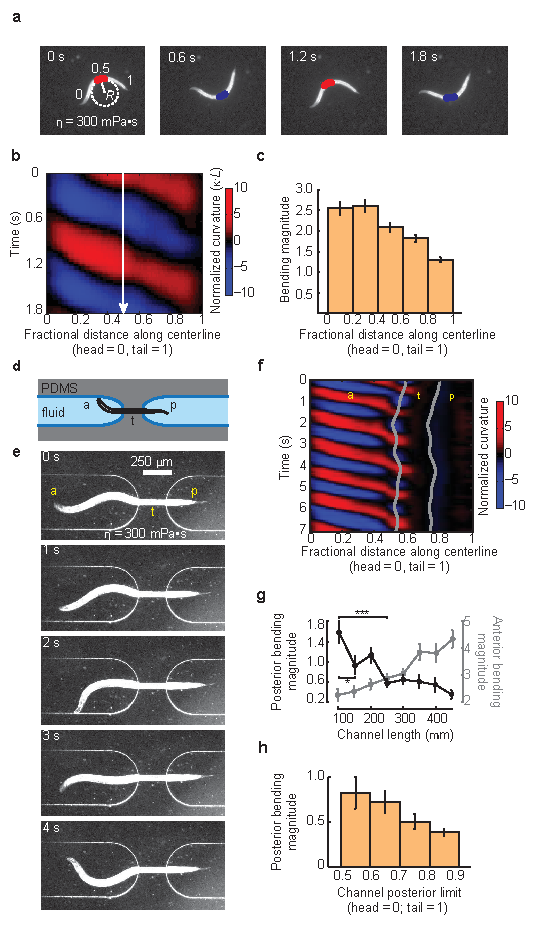
\includegraphics[width=\textwidth]{figures/proc1}
\caption[Bending of posterior regions requires anterior bending. ] {Bending of posterior regions requires anterior bending. (\textbf{a}) Video images of a worm swimming forward. Bending is quantified by measuring the radius 	of curvature R at each point along the centerline. Position along the centerline is measured in normalized coordinates using the fractional distance from head to tail (head $= 0$; tail $= 1$). A red-blue colormap illustrates alternating curvatures at fractional distance $= 0.5$. (\textbf{b}) Kymograph of time-varying curvature illustrating retrograde bending waves along the worm represented in non-dimensional units. To do this, the curvature at each point along the centerline, $\kappa = 1/R$, is multiplied by worm length, $L$. (\textbf{c}) Bending magnitude along the body of a wide-type free swimming worm, measured as the standard deviation of normalized curvature over time. $n = 18$ worms, mean $\pm$ one standard error. (\textbf{d}) Schematic of microfluidic device. a stands for anterior region, p stands for posterior region, and t stands for trapped region of a worm.  (\textbf{e}) Video images of a wide-type young adult worm exhibiting forward undulatory gait inside the microfluidic device (also see Supplementary Movie 1). The channel divides the worm body into unrestrained anterior, posterior, and trapped middle regions. (\textbf{f}) Kymograph of time-varying curvature along the body of the worm shown in (\textbf{e}). Gray lines mark the anterior and posterior limits of the straight channel. (\textbf{g}) Bending magnitude of a posterior and an anterior body region ($\sim 0.15$ worm length) adjacent to the channel, measured as the standard deviation of time-varying normalized curvature, is plotted as a function of the length of the trapped region. $n \geq 10$ worms for each condition, mean  $15$	$\pm$ one standard error. Position of the posterior limit of the channel is $0.7 \pm 0.1$ (mean $\pm$ standard deviation) for each condition, measured as the fractional distance from head to tail. *$P<0.05$, ***$P = 0.0001$, Mann-Whitney U test.  (\textbf{h}) Bending magnitude of a posterior body region (mean $\pm$ one standard error) as a function of the position of the posterior limit of the channel. We measured 64 bouts of forward movement trapped in different channel positions from $20$ worms. Channel length is $300 \mu$m.\label{fig:proc1}}
\end{FPfigure}



First, we sought to determine whether the motor activity in one body region might depend on the 
bending of neighboring body regions. To test this, we designed microfluidic devices that enabled 
us to immobilize body regions of varying length along the middle of a young adult worm (Fig.~\ref{fig:proc1}d-e and Supplementary Movie 1). Our first device trapped the center of a worm in a narrow 
straight channel. The region of the worm's body inside the channel was restrained, while  regions of the worm's body either anterior or 
posterior to the channel were free to bend (Fig.~\ref{fig:proc1}d-e). We used a channel diameter ($40 \mu$m) that was sufficient to 
immobilize the trapped region (worm diameter is $54 \pm 4 \mu$m; mean $\pm$ SD) with minimum 
constriction.  

We consistently recorded bouts of forward movement ($> 10$ s) when we set the posterior limit of 
the channel at $0.7 \pm 0.1$ in fractional worm length along the body. Bending waves would 
propagate normally to the anterior limit of the channel (gray data points in Fig.~\ref{fig:proc1}g). Short 
channels ($100 \mu$m long) did not affect wave propagation along the worm body; the bending wave 
that emerged from the posterior limit of the channel (black data points in Fig.~\ref{fig:proc1}g) exhibited 
similar amplitude as a free swimming worm (Fig.~\ref{fig:proc1}c). However, increasing channel length 
beyond $200 \mu$m significantly diminished the bending amplitude in the posterior body region (Fig.~\ref{fig:proc1}1e-g). Fixing the channel length, but moving it towards the tail also reduced the posterior 
bending amplitude (Fig.~\ref{fig:proc1}h, $R = -0.24$, $p < 0.05$, Spearman’s rank correlation test).




\section{Manuscript Information}
\subsection{Submitted for publication as}
A previous version of this chapter was submitted as \citep{wen_bending_2011}:

\bibentry{wen_bending_2011}

\subsection{The Author's Contribution}
The overwhelming majority of the work in this chapter was performed by Quan Wen. Andrew M.~Leifer assisted with optogenetic experiments and provided technical support regarding microscopy and experimental design. Additionally, Andrew made major contributions to the analysis software. 

The majority of the manuscript was written by Quan Wen and Aravinthan D.T.~Samuel.
